%Tex file for Git Hub for Authors HOWTO
\documentclass[a4paper, 12pt]{article}
\usepackage{graphicx}
\title{Git and GitHub for Authors}
\author{TM Coker}
\setlength{\parskip}{1ex}
\setlength{\parindent}{0em}
%set of macros to adjust page layout
\pdfpagewidth=\paperwidth 
\pdfpageheight=\paperheight
\setlength{\marginparwidth}{20mm}
\setlength{\hoffset}{-1in}
\setlength{\voffset}{-1in}
\setlength{\textwidth}{167mm}
\setlength{\textheight}{262mm}
\setlength{\oddsidemargin}{20mm}
\setlength{\evensidemargin}{20mm}
\begin{document}
\maketitle
\section{Introduction}
\subsection{What is Git and GitHub}
Git is a software source control system, initially written by Linus Torvalds specifically to support Linux kernel development, the assessment being that other systems then available were not up to the demands of Limux development. Development was started in 2005 and Git is now open--source software distributed under the GNU GPL.

In common with other systems Git provides the means for:
\begin{itemize}
\item Many programmers to collaborate on a single software application.
\item Manage release and software version control.
\item Track changes to software as it is developed.
\item Branch a code base to allow specific issues to be worked on in parallel.
\item Merge branches back into the main code base.
\end{itemize}

Git also has a similar top level structure to other solutions -- projects or applications roughly correspond to `repositories' (often called `repos'). Within any one repo there will exist a number of branches, and typically in software development a branch represents a version of the code being developed to address one specific issue, which could be a new feature or fixing a bug. The key feature of such systems is that they maintain a full record of changes to all files that are held within the repo, for software this is required for tracking purposes, e.g. who made what change when, but it also provides a complete history of the software as it has been developed.

GitHub is effectively a cloud based implentation of Git, with a browser based interface into the more sophisticated functions, such as `pull requests', code reviews, merging, release management and so on (none of which really concern authors). However GitHub cannot effectively be used on it's own, it really needs a local Git implementation and as such, for our needs, Git Hub is really just cloud storage (although it does offer some facilities that your local Git application doesn't have).

\subsection{Relevance to Authors}
Authors, although they are not writing software, have similar requirements to software engineers:
\begin{itemize}
\item They develop source material in an incremental way, keeping track of changes and version information.
\item In many cases, particularly in the sciences, several authors will be collaborating on a single book, article or paper, in which case simple word processing software such as Word is limited, as is LaTex. Although alternatives such as Google Docs can be used, even these have their limits, particularly for laying out scientific papers with cross--referencing, citations and so on.
\item For authors using LaTex, because of it's sophistication, other than file backup software, there is no obvious solution to the need for revision control, archiving and so on.
\item Authors need to periodically archive and/or back up their material.
\item They would preferably back up to cloud storage as well as any local media - local hard--drives, additional home file storage and so on.
\item If necessary they may want to work on two or more versions of essentially the same document.
\item They may want to retrieve an older version of the source material, either by rolling back changes or retrieving a complete set of course material that has been suitably labelled.
\end{itemize}
All these requirements are essentially the same as the ones software engineers have when writing code, although authors only need a modest subset of the full set of features that Git or any other source control system provides. However the general message is that a system like Git/GitHub has many of the features that author's look for, indeed (as we'll see below) there are setup files designed specifically for Tex/LaTex, which is a document authoring system many authors, particularly in the sciences, use.

\subsection{Technical Description}
This is not in any way a full description of the inner workings of Git, but part of the purpose of this document is to explain why you might want to use Git/GitHub when you aren't already.

Unlike many equivalent systems, Git does not primarily use a client/server model, the entire system can be deployed to a single machine, although collaboration facilities would clearly be limited. In practice Git can be considered as a private file system with a set of coded utilities running on top. The utilities manage files within repos and branches, storing files, tracking changes and so on. Git has been primarily written to run on Linux and the actual user interface has always been the command line. However the system has become so successful that there are many third party applications that provide a traditional window based GUI. A little bit of web searching will quickly lead you to many examples, e.g. GitKraken, SmartGit, Fork and so on. A quick online search for `git gui' will quickly lead you to a plethora of alternatives, but be aware many are not free, or have proprietary licences or hidden drawbacks.

Notwithstanding the above, two particular implementations should be considered:
\begin{itemize}
\item Git For Windows -- this is effectively the `official' Windows version from the open--source collaboration that maintains and develops Git.
\item GitHub Desktop - assuming that you're intending to use GitHub, then GitHub Desktop seems an obvious solution for ease of integration. Open source, free and available under the MIT Licence, with reasonably good support and also a thriving community.
\end{itemize}
As a little bit of context, I'd not suggest GitHub Desktop as first choice client for actual coding. When I was last running a software team, we actually settled on Fork (whcih is not free). However for the more limited needs of authors I'd suggest that GitHub Desktop is more than adequate. As you'll see below, this is the solution that has been used by the author for this document.

\section{Getting Setup with Git and GitHub}
There are two principle steps to getting set up -- registering and creating a GitHub account, and installing your local Git application. These two can actually be done quite independently and I'd suggest you get up and running with your local Git application before setting up on Git Hub. This is particularly the case if you decide to use GitHub Desktop as this makes for a very easy process to `push' your local repos up to GitHub. The alternative workflow is to create repos on GitHub then clone them to your local machine, which works fine and is only marginally more comlex. Whichever way ou end up doing it, there is a process to link your Git application to GitHub, this is fairly straightforward if you're using GitHub desktop and is another reason to use this application.

\subsubsection{Assumptions}
For the rest of this guide, it is assumed that you are using:
\begin{itemize}
\item Windows 10.
\item GitHub Desktop.
\item You are using LaTex to create your documents, MiKTex version 2.9.
\item And you are setting up GitHub desktop before registering on GitHub.
\end{itemize}
If that is not the case, it doesn't necessarily mean that you can't use this guide, the broad steps to take should be the same regardless of actual implementation, but the screengrabs in particular will be of limited use.

\subsection{Installing and Running GitHub Desktop}
Once you've downloaded the installer run it a snormal, the installation process is simple and direct and should launch the application straight away. Once its running you should see the following window (Figure \ref{startscreen})
\begin{figure}
\centering
\includegraphics[width=\linewidth]{startscreen}
\caption{Start screen for GitHub Desktop}
\label{startscreen}
\end{figure}
They following steps will set up a repo, initialise it with a tex file, make the initial `commit', build the document and make a second `commit' after the build.
\begin{enumerate}
\item Click the `Create New Repository' option, this will give you a new dialogue - Figure \ref{newrepo}. Fill int the details as required. Initialising with a README file is not essential but good practice. If you are using LaTex then click the crop down against `GitIgnore' and select `Tex'.
\end{enumerate}
\begin{figure}
\centering
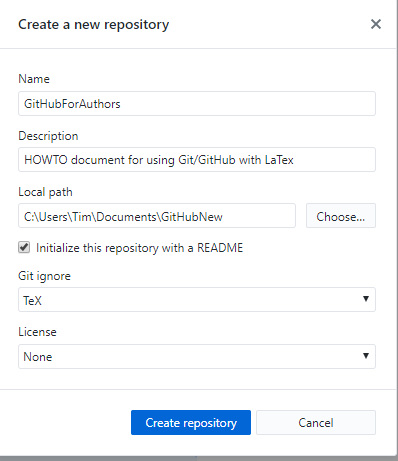
\includegraphics{NewRepo}
\caption{Dialogue to create a new repo.}
\label{newrepo}
\end{figure}







\end{document}